% !TeX spellcheck = en_US
\section{Problem 11}
Convolutional Neural Networks (CNNs) have revolutionized in the field of image processing and computer vision and are widely utilized.\\

In this exercise we are considering a $6 x 6$ image I, where each entry represents the intensity of a pixel.The values are typically normalized , and the CNN would perform operations on this matrix to learn features and perform tasks like classification, detection, or segmentation. We will apply various layers and filters, so that we can extract higher-level features.\\


\begin{equation}
	I = \begin{bmatrix}
		20 & 35 & 35 & 35 & 35 & 20 \\
		29 & 46 & 44 & 42 & 42 & 27 \\
		16 & 25 & 21 & 19 & 19 & 12 \\
		66 & 120 & 116 & 154 & 114 & 62 \\
		74 & 216 & 174 & 252 & 172 & 112 \\
		70 & 210 & 170 & 250 & 170 & 110 \\
	\end{bmatrix}
\end{equation}
\label{fig:input_image}

Given the input matrix we can understand that it represents a grayscale image. In a grayscale image, each pixel is represented by a single intensity value, typically on a scale $\left[0, 255\right]$. The 2D input array contains such intensity values for each pixel in the image.

\subsection{Question A}
The output of a convolution layer is a new matrix that's the result of the convolution operation. The convolution operation involves sliding the kernel over the input matrix, with a given stride $\left(1,1\right)$, and for each position, computing the sum of elementwise multiplications. \\

The use of a stride in a convolutional layer is important, because it determines how much the filter or kernel moves across the input matrix. In our case, a stride of $\left(1,1\right)$ means that the kernel moves one step at a time horizontally and vertically. This will result in an output matrix that is smaller than the input matrix by one less than the kernel size in each dimension. So, in our case the output will be a $4 x 4$. Also,the output's matrix size is smaller than the original because of the "valid" mode on our code. The "valid" mode means that the convolution product is only given for points where the kernels overlap completely with the input array. It doesn't add any padding to the input image.\\

In addition, the kernel we have defined is a $3 x 3$ matrix with a zero in the center. This means that the convolution operation will sum up the values of the eight surrounding pixels and ignore the center pixel for each position in the input image.\\

So, in conclusion, with a
\begin{itemize}
	\item $stride = \left(1,1\right)$ and 
	\item $	kernel = \begin{bmatrix}
		1 & 1 & 1  \\
		1 & 0 & 1  \\
		1 & 1 & 1  \\
	\end{bmatrix}$
\end{itemize}

The result of the convolution is a $ 4 x 4$ matrix\\

\begin{equation}
	result = \begin{bmatrix}
		225 & 258 & 250 & 209  \\
		458 & 566 & 552 & 472  \\
		708 & 981 & 887 & 802  \\
		1000 & 1488 & 1320 &1224 \\
	\end{bmatrix}
\end{equation}
\vspace{6mm}

The resulting matrix, represents the features in the input image that the kernel was able to detect. In this case, the kernel seems to act like a filter that emphasizes the surrounding context of each pixel. The exact interpretation would depend on the specific values in the input image and the kernel. 

\begin{figure}[H]
	\centering
	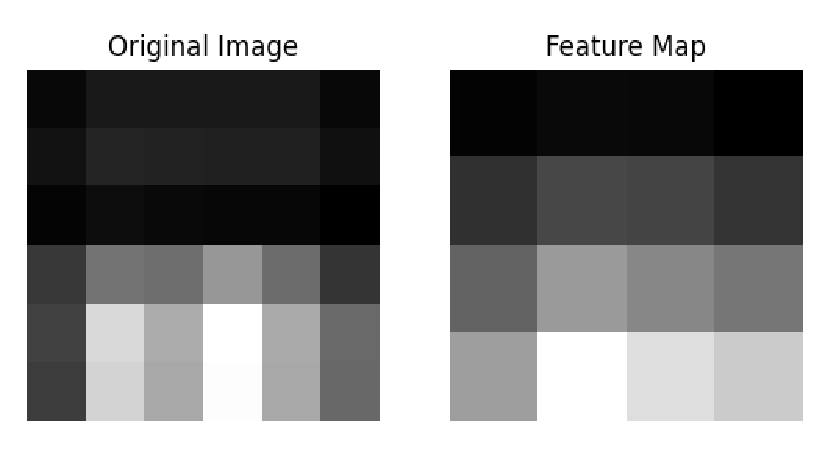
\includegraphics[width=.7\textwidth]{../Problem 11/conv_result.pdf}
	\caption{The Original Image and the Image after the convolution}
\end{figure}
\vspace{3mm}
\subsection{Question B}
Now, using the output of the convolution of the input image we are going to apply a max pooling layer with the following properties: 
\begin{itemize}
	\item $stride = \left(2,2\right)$ and 
	\item $	window\ \ shape = \left(2, 2\right)$
\end{itemize}
In general, a max pooling layer performs a downsampling operation along the spatial dimensions, width and height, of the input data. The main goal is to reduce the dimensionality of the input, which helps to control overfitting and reduces computational complexity for subsequent layers.\\
In our exercise, the size of the input matrix is reduced from $ 4 x 4 \rightarrow 2 x 2$.\\
 
The max pooling operation works by defining a spatial neighborhood, in our case a $ 2 x 2\ \ window$ and taking the maximum element from the rectified feature map within the window. This window is slid over the input data with a certain stride to produce a new matrix where each element is the maximum of a neighborhood from the input. This process effectively reduces the spatial dimensions of the feature map.\\

The result of the max pooling layer is a $2 x 2$ matrix of the same image
\begin{equation}
	max\_pooling = \begin{bmatrix}
		566 & 552   \\
		1488 & 1320 &  \\
	\end{bmatrix}
\end{equation}
\\
We can conclude that the max pooling operation only reduces the size of the feature map while preserving the most important and prominent features. It gives a more abstract and compressed representation of the input image.
\vspace{3mm}

\subsection{Question C}
As we have seen in the previous questions, the use of kernels, also known as filters, is a fundamental tool for image processing. They are essential for the efficient extraction of different features, the reduction of the number of parameters and optimal processing. In this exercise, we will emphasize the importance of kernels for extracting different features from the same input image.\\

So, for the input image \ref{fig:input_image} we have the following results:
\begin{itemize}
	\item \underline{Filter F1}\\
	
\end{itemize}





